\documentclass[10pt,
			   xcolor=svgnames,
			   hyperref={linkcolor=red, citecolor = DarkGreen, colorlinks=true, urlcolor=Navy}]{beamer}
			   
\usepackage[english]{babel}
\usepackage[utf8x]{inputenc}

\usepackage{tikz}
\def\checkmark{\tikz\fill[scale=0.4](0,.35) -- (.25,0) -- (1,.7) -- (.25,.15) -- cycle;}

\mode<presentation>
{
  \usetheme{Copenhagen}      % or try Darmstadt, Madrid, Warsaw, ...
  \usecolortheme{beaver}
} 

\usepackage{multicol}
\setlength{\columnseprule}{0.pt}

\usepackage{float}
\usepackage[authoryear]{natbib}

\graphicspath{{./pic/}}

\usepackage[font=scriptsize, center]{caption}

%%% Commandes utiles définies
\newcommand{\argmin}{\mathop{\mathrm{argmin}}}

\newcommand{\bepar}[1]{
	\left( #1 \right)  
}
\newcommand{\becro}[1]{
	\left[ #1 \right]  
}

\newcommand{\norm}[1]{
	\left \vert \left \vert #1 \right \vert  \right \vert
}

\usepackage{siunitx}

\usepackage{pifont}
\newcommand{\bwarrow}{\item[\color{DarkRed} \ding{227}]}
\newcommand{\warrow}{\item[\color{blue!50!black!70} \tiny{\ding{109}}]}
\newcommand{\sarrow}{\item[\color{blue!50!black!70!orange!60} \tiny{\ding{55}}]}


\usepackage{geometry}
\geometry{hmargin=1.cm, vmargin=0cm}

\xdefinecolor{bviolet}{named}{BlueViolet}

%%%%%%%%%%%%%%%%%%%%
%%% Couleurs %%%
\xdefinecolor{brick}{named}{DarkRed}
\xdefinecolor{navy}{named}{Navy}
\xdefinecolor{midblue}{named}{MidnightBlue}
\xdefinecolor{dsb}{named}{DarkSlateGray}
\xdefinecolor{dgreen}{named}{DarkGreen}

%%% 	Raccourcis 	%%%
\newcommand{\keps}{$k-\varepsilon$}
\newcommand\bk{\color{black}}
\newcommand\brick{\color{brick}}
\newcommand\navy{\color{navy}}
\newcommand\midblue{\color{midblue}}
\newcommand\dsb{\color{dsb}}
\newcommand{\dgreen}{\color{dgreen}}
\newcommand\red{\color{red}}

\usepackage{setspace}

    \expandafter\def\expandafter\insertshorttitle\expandafter{%
       \insertshorttitle\hfill%
       \insertframenumber\,/\,\inserttotalframenumber}

% Things for first slide :
\title[Machine learning in Physics fields]{An attempt to learn Physics : ML in fluid mechanics problems}
\author{Saura Nathaniel (PHD Student)\\}

\date{$5^{\text{th}}$ July 2018}
\institute{\bf LMFL
\begin{center}
	\begin{minipage}[!ht]{0.9\textwidth}
	\centering
	
\includegraphics[scale=0.75]{logo_lmfl_border.png}
	\end{minipage}
\end{center}
}

% Begin 
\begin{document}
\begin{frame}
  \titlepage
\end{frame}

\begin{frame}{Main idea through few observations}

\begin{block}{Well known question : cost computation or precision ?}
\begin{itemize}
\item[$\bullet$] DNS provides perfect solutions but needs a lot of time computation
\item[$\bullet$] RANS models provide quicker more or less precise results 
\end{itemize} 
\end{block}
\vspace{1cm}
\begin{block}{ML algorithms exploding development (in every field)}
\begin{itemize}
\item[$\bullet$] Gaussian Process
\item[$\bullet$] RForests, NNetworks (Supervised) for classification or regression tasks (more and more papers in fluid mechanics)
\item[$\bullet$] Reinforcement Learning (few papers in fluid mechanics so far)
\end{itemize}
\end{block}

\end{frame}

\begin{frame}{Main idea through few observations}
\begin{block}{Different implementations}
\begin{itemize}
	\item[$\bullet$] Data-Driven augmentation (use of high fidelity datasets) with a combination of Bayesian Inference and Gaussian Process (or other ML methods)
	\item[$\bullet$] Machine Learning to fully recover physical behaviour
\end{itemize}
\end{block} 

\tableofcontents

\end{frame}

\section{Bayesian inversion framework (BIF)}
\begin{frame}{Infer beta through inversion}
\begin{block}{Modified closure equation }
The main idea of RANS models is to add a closure equation. The main idea of BI is to add a flexible term in this closure to correct the error injected.  
\center{$\displaystyle \mathcal{F}\bepar{\color{BlueViolet} \beta(\mathbf{x}, t) \bk P_{\text{roduction}}  , D_{\text{issipation} }, T_{\text{ransport}}} = 0 $}
\end{block}
$$ \beta_M = \argmin \mathcal{J}$$
$$\mathcal{J} = \becro{\frac{1}{2} \bepar{\text{Obs} - h\bepar{\beta}}^T\textbf{C}^{-1}_m\bepar{\text{Obs} - h\bepar{\beta}} + \bepar{\beta - \beta_{\text{p}}}^T\textbf{C}_\beta^{-1}\bepar{\beta - \beta_{\text{p}}}}$$

\begin{block}{Importance and meaning of $\beta$}
\begin{itemize}
\item[$\bullet$] Discrepancy vector minimizing the distance between DNS and RANS solutions (can be seen as a vector of latent variables)
\item[$\bullet$] Maximizing $\color{BlueViolet} \beta \bk | \text{Obs}$ 
\end{itemize}
\end{block}

\end{frame}
\begin{frame}{Bayesian Inversion Framework (BIF)}
Framework proposed by Duraisamy \textit{et. al} in \citep{parish2016paradigm}
\begin{multicols*}{2}
\noindent
	\begin{figure}[!ht]
	\centering
	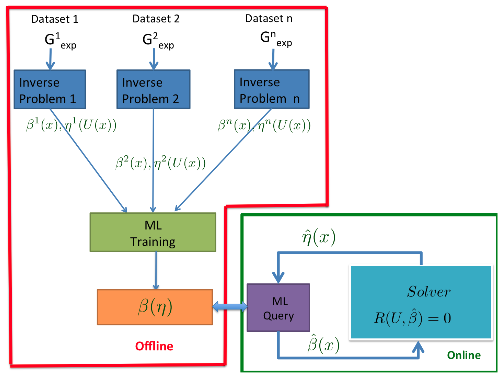
\includegraphics[scale=0.3]{singh.png}
	\caption{Figure extracted from \citep{singh2017machine}}
	\end{figure}
	
	\columnbreak

	\begin{itemize}
	\item[1 --] Infer descrepancy \color{BlueViolet} \textit{information} \bk $\beta$ as the MAP solution \\[5mm]
	
	\item[2 --]	\textit{Generalize} this information using ML methods to have a \color{BlueViolet} \textit{knowledge} \bk: $\beta = \mathcal{F}\bepar{\eta_1, \eta_2,...}$ \\[5mm]
 
	\item[3 --] Inject ML predicted correction into model's equation(s) \\[5mm]
	
	\end{itemize}
			
\end{multicols*}
\end{frame}

\begin{frame}{BIF example : 1D heat conduction with radiative and conductive heat sources}
\begin{block}{Real and Model equations}
\begin{itemize}
\item[$\bullet$] Real equation :
\begin{center}
$\displaystyle \frac{d^2T}{dz^2} + \varepsilon(T)\bepar{T^4_\infty - T^4} + h\bepar{T_\infty - T} = 0$
\end{center}
\item[$\bullet$] Model equation :
\begin{center}
$\displaystyle \frac{d^2T}{dz^2} + \varepsilon_0\color{BlueViolet}\beta(z)\bk\bepar{T^4_\infty - T^4}= 0$
\end{center}
\end{itemize} 
\end{block}

\begin{itemize}
\item[\dgreen \checkmark] BFGS method to minimize $\mathcal{J}$ $\rightarrow$ $\beta_{\text{MAP}}$ \& $\text{Hess}^{-1}_{\beta_{\text{MAP}}}$
\item[\dgreen \checkmark] Create $\beta_{\text{final}}$ distribution : \\
\begin{center}
$ \beta_{\text{final}} \equiv \beta \sim \mathcal{N}\bepar{\beta_{\text{MAP}}, {\text{Hess}^{-1}_{\beta_{\text{MAP}}}}}$
\end{center}
\end{itemize}

\end{frame}

\begin{frame}{BIF : Few figures based on inversion ($T_\infty = \ang{15}$C)}
\begin{multicols}{2}
\noindent
	\begin{figure}[H]
	\centering
	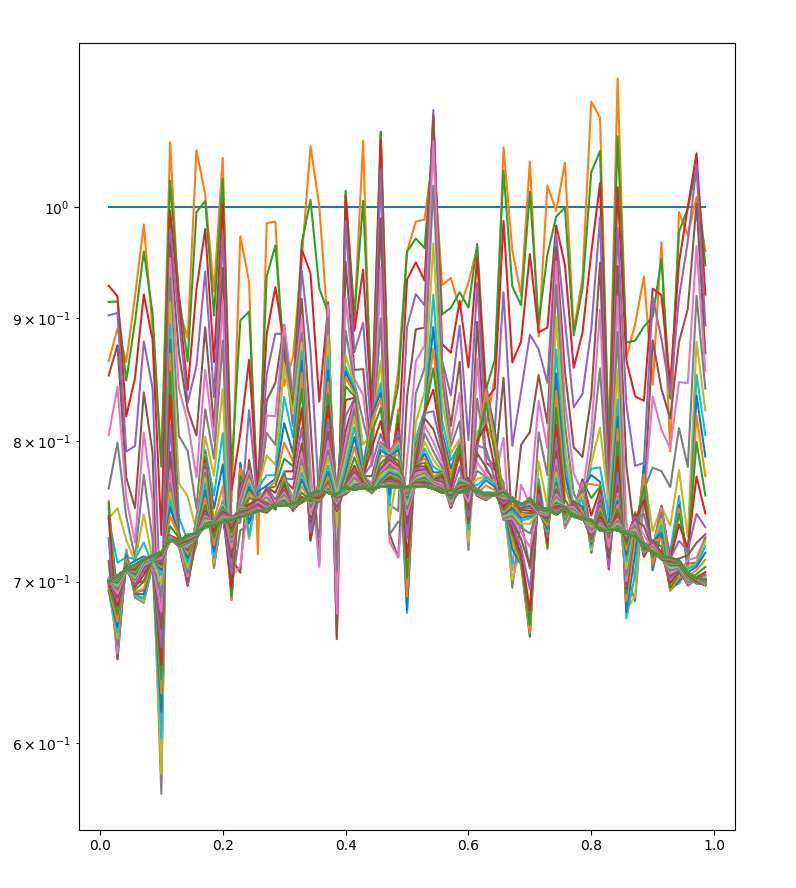
\includegraphics[scale=0.25]{Pres_Evolution_beta_map.png}
	\caption{Evolution of beta through the minimization process}
	\end{figure}

\columnbreak
	
	\vspace*{-1cm}
	\begin{figure}[H]
	\centering
	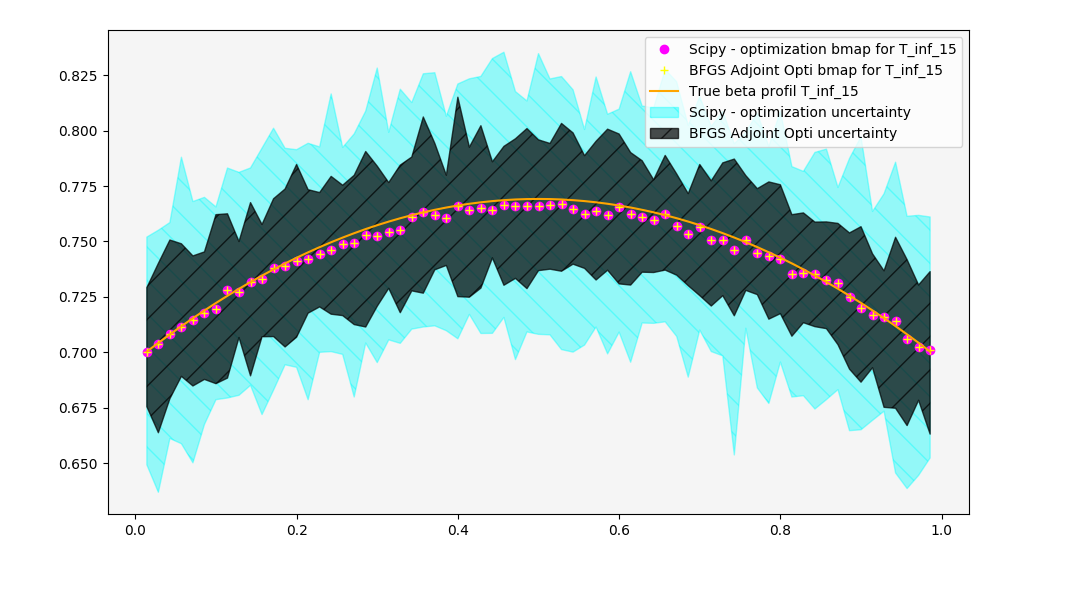
\includegraphics[height=4cm, width=6cm]{Pres_T_15_Full_Beta_Comp.png}
	\end{figure}
	
	\vspace*{-2.5cm}
	\begin{figure}[H]
	\centering
	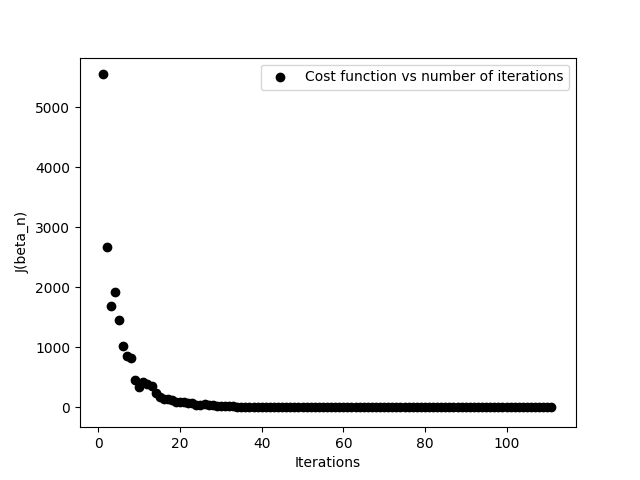
\includegraphics[height=4cm, width=6cm]{Evolution_de_l'erreur_T_inf_15.png}
	\end{figure}		


	
\end{multicols}
\end{frame}

\begin{frame}{BIF : Next Step : Machine Learning}
Reproduce the previous calculs for T = 5:5:50 \\[1cm]

Construction $X$ and $y$ in $\mathcal{D} = \left\lbrace \ \underbrace{\bepar{T_{\text{inf}},T(x_i)}}_{X_i}, \ \underbrace{\beta_i}_{y_i}\ \right\rbrace$ for each T.\\
In matrix notation : 

\begin{multicols}{2}
\noindent
$$ X = \left[ \begin{array}{c} \cdot \\ \cdot \\ T_{\text{inf}},\ T(x) \\ \cdot \\ \cdot
			  \end{array}
	   \right]
$$
\columnbreak
$$ y = \left[ \begin{array}{c} \cdot \\ \cdot \\ \beta(x) \\ \cdot \\ \cdot
			  \end{array}
	   \right]
$$
\end{multicols}
Neural Network generalization : \\
\begin{center}
 $\beta_1(x), ..., \beta_n(x) \rightarrow \beta_{\text{ML}} = \mathcal{F}\bepar{\eta_1 = T_{\text{inf}}, \eta_2= T}$
\end{center}
\end{frame}

\begin{frame}{(BIF) : Prediction with NN }
$T_\infty = \ang{28}$C 
\begin{figure}[H]
	\centering
	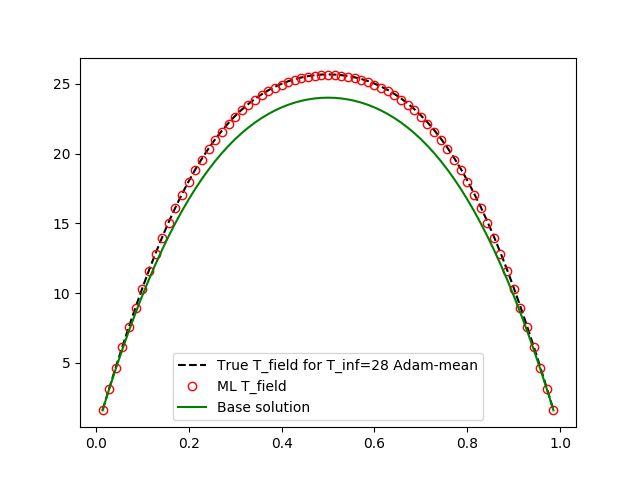
\includegraphics[scale=0.5]{T_True_vs_T_ML_N_sample_5_T_inf_28_Adam-mean.png}
\end{figure}

\end{frame}

\begin{frame}
$T_\infty = \ang{55}$C 
\begin{figure}[H]
	\centering	
	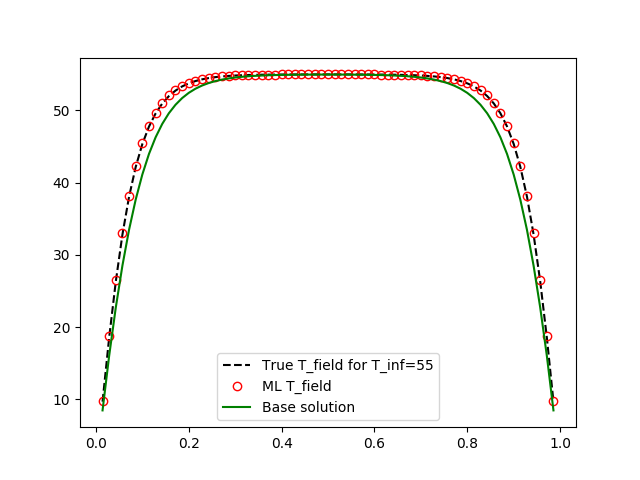
\includegraphics[scale=0.5]{TBeta_True_vs_TBeta_ML_N_sample_=_5_T_inf_=_55.png}
\end{figure}

\end{frame}

\begin{frame}
$T_\infty = 35 + 20\sin(2\pi x)$ 
\begin{figure}[H]
	\centering	
	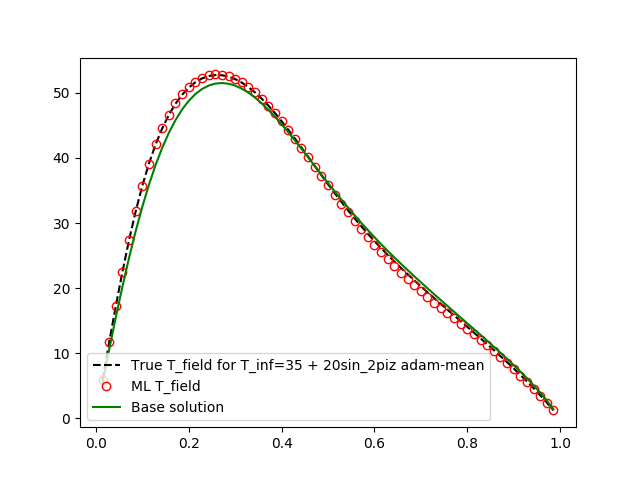
\includegraphics[scale=0.5]{T_True_vs_T_ML_N_sample_5_T_inf_35_+_20sin_2piz_adam-mean.png}
\end{figure}
\end{frame}


\begin{frame}{(BIF) Viscous Burgers Equation 1D}
	
	\begin{block}{Equations}
		\begin{itemize}
			\item[$\bullet$] Real equation :
				\begin{center}
					$\displaystyle \frac{\partial u}{\partial t} + u \frac{\partial u}{\partial x} - \frac{\partial^2 u}{\partial x^2} = 0$
				\end{center}
			\item[$\bullet$] (Inference) Model equation (1) :
				\begin{center}
					$\displaystyle \frac{\partial u}{\partial t} + u \color{BlueViolet} \beta(x,t) \bk - \frac{\partial^2 u}{\partial x^2} = 0$
				\end{center}
		\end{itemize} 
	\end{block}

	\begin{itemize}
		\item[\checkmark] Real solution obtained with Lax Wendroff Scheme
		\item[\checkmark] Infered solution obtained with Crank Nicholson Scheme
		\red \item[\red \checkmark \bk] One inference at each time iteration \bk
	\end{itemize}

\end{frame}

\begin{frame}{(BIF) VBE 1D : Inference step}
	\begin{block}{A look at the future}
		At each iteration $n$ we compute the $\beta_{\text{MAP}}$ minimizing a cost function that depends on the solution at $n+1$ : \\ 
		\begin{center}
			$\displaystyle \mathcal{J}^n = \frac{1}{2} \bepar{\Delta_{_{\text{LW-CN}}}U^{n+1}}^T \text{C}_\text{obs}^{-1} \bepar{\Delta_{_{\text{LW-CN}}}U^{n+1}} + \lambda \bepar{\beta^n -
			\beta_{\text{p}}}^T \text{I}_d \bepar{\beta^n - \beta_\text{p}}$
		\end{center}
		Where $\Delta_{_{\text{LW-CN}}}U^{n+1} = \bepar{U^{n+1}_{\text{obs}}}^\text{LW} - \bepar{U^{n+1}_\beta}^\text{CN}$\\
		And \\
		\begin{center}
			$\displaystyle \beta_{\text{MAP}}^n = \argmin \mathcal{J}^n$
		\end{center}
	\end{block}
	
	\begin{itemize}
		\item[\checkmark] Initialize the problem with $u_0(x,t) = \sin((2\pi x)/L)$ in L-length domain
		\item[\checkmark] Periodic boundary condition
	\end{itemize} 
\end{frame}

\begin{frame}{(BIF) VBE 1D : Inference step (figures)}
\vspace{-1cm}
\begin{multicols}{2}
\noindent
	\begin{figure}[H]
		\centering
		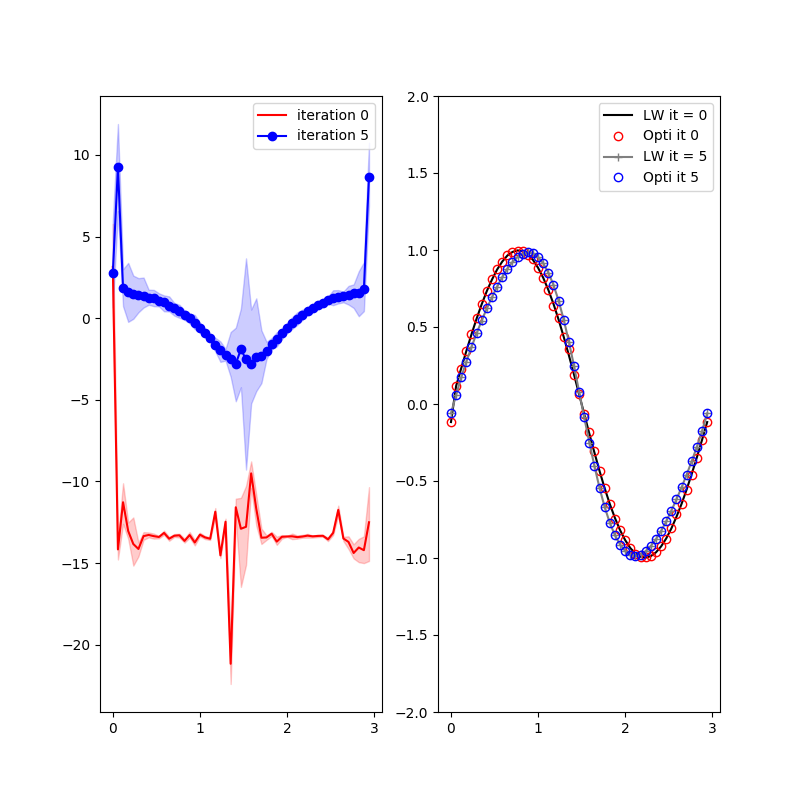
\includegraphics[width = 6cm, height= 6cm]{nu0_0250_CFL0_40_Nx_52_InferenceVSTrue_it5.png}
		\vspace{-0.5cm}	
		\caption{Left : Beta at time $n$ Right : Comparaison between reel solution and inferred solution at iteration 1(red) and 6(blue)}
	\end{figure}

\columnbreak

	\begin{figure}[H]
		\centering
		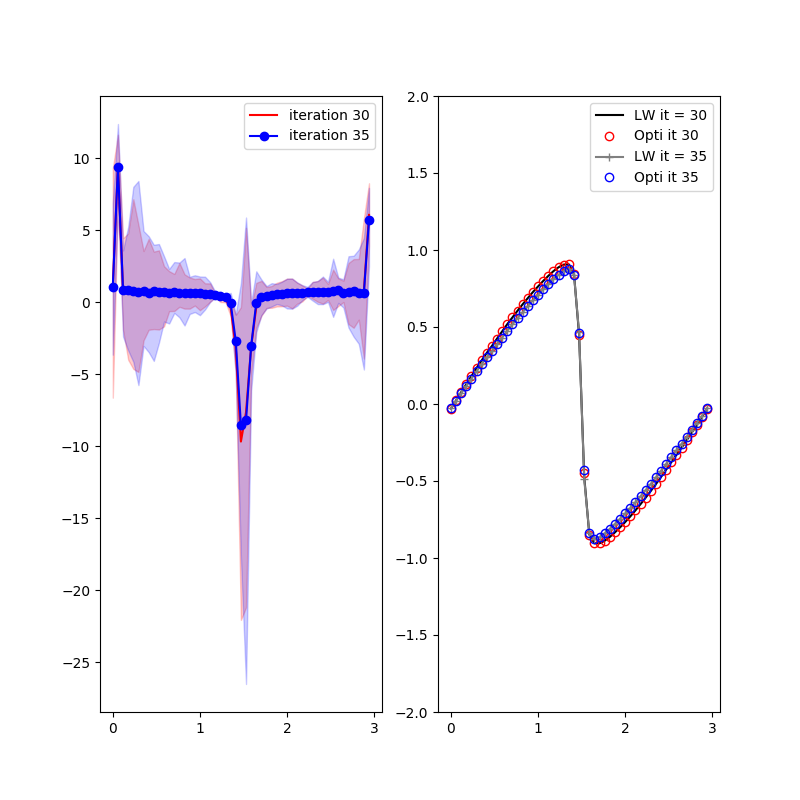
\includegraphics[width = 6cm, height=6cm]{nu0_0250_CFL0_40_Nx_52_InferenceVSTrue_it35.png}
		\vspace{-0.5cm}	
		\caption{Left : Beta at time $n$ Right : Comparaison between reel solution and inferred solution at iteration 31(red) and last(blue)}
	\end{figure}

\end{multicols}

\end{frame}


\begin{frame}{(BIF) VBE 1D : Machine Learning step}
	More difficult now : what are $\eta$ to use in $\beta = \mathcal{F}(\eta)$ ?
	\begin{itemize}
		\item[$\bullet$]$\beta^{n+1} = \bepar{U_{i-1}^n, U_i^n, U^n_{i+1}}$ 
		
		\item[$\bullet$] $\beta^{n+1} = \bepar{X_{i-1}^n, X_i^n, X^n_{i+1}, U_{i-1}^n, U_i^n, U^n_{i+1}}$ 		
		
		\item[$\bullet$] $\beta^{n+1} = \bepar{X_{i-1}^n, X_i^n, X^n_{i+1}, 
		U_{_{\bk i-1}}^{\red n-1}, U_{\bk i}^{\red n-1}, U_{_{\bk i+1}}^{\red n-1}, 
		U_{i-1}^n, U_i^n, U^n_{i+1}}$ 		
		
		\item[$\bullet$] \scriptsize$\beta^{n+1} = \bepar{X_{i-1}^n, X_i^n, X^n_{i+1}, 
		U_{_{\bk i-1}}^{\navy n-2}, U_{\bk i}^{\navy n-2}, U_{_{\bk i+1}}^{\navy n-2},
		U_{_{\bk i-1}}^{\red n-1}, U_{\bk i}^{\red n-1}, U_{_{\bk i+1}}^{\red n-1}, U_{i-1}^n, U_i^n, U^n_{i+1}}$ 		\\[0.54cm]
	\end{itemize}
	\normalsize

	Problem linked to this framework :
	\begin{itemize}
		\sarrow Inversion can take long time to give $\beta_{\text{MAP}}$
		\sarrow The need to produce various inferences to construct wide datasets
	\end{itemize}
	
	\begin{exampleblock}{Idea}
		Can we use NN brute force to infer the behaviour of U through time ?
	\end{exampleblock}	
	No more inference needed
\end{frame}

\section{Neural network brute force (NNBF)}
\begin{frame}{Building the datasets}

	\begin{itemize}
		\item[$\bullet$] Different sinusoides as initial conditions

		\begin{itemize}
			\sarrow Different amplitudes (between 1 and 2) -- 15 cases
			\sarrow Random phases
 		\end{itemize}
	
	\begin{figure}[H]
		\vspace{-0.3cm}		
		\centering
		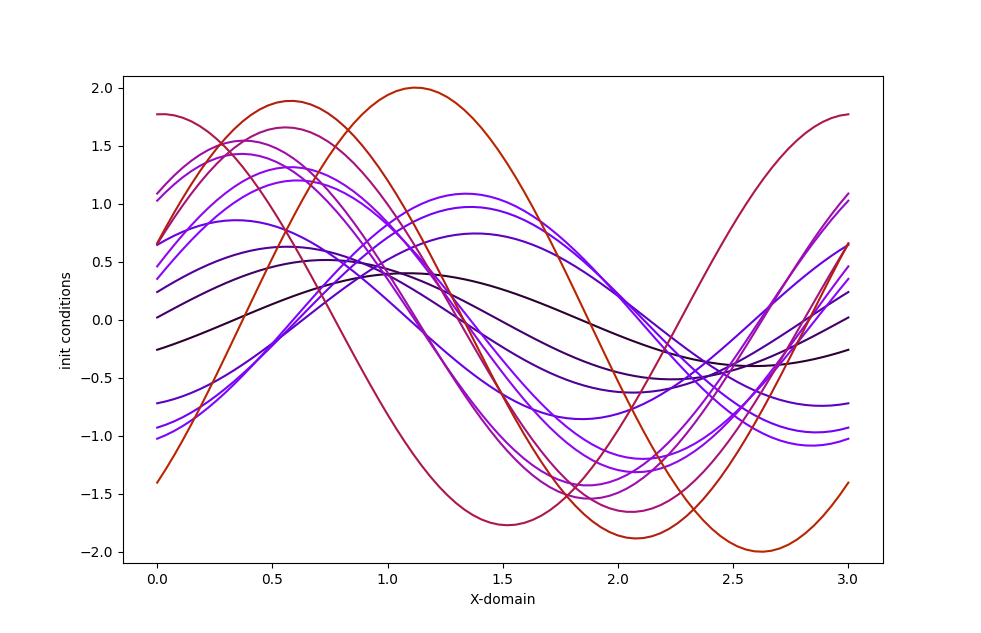
\includegraphics[scale=0.3]{Initialisation_cases.png}
	\end{figure}			
		
 		\item[$\bullet$] Lax Wendroff scheme to solve each initial condition
	\end{itemize}
\end{frame}

\begin{frame}{Strategy employed here}
	We want to find the functionnal linking the solution $U^{n+1}$ and some n$^{\text{th}}$ parameters :\\
	\begin{center}
	$ \displaystyle U^{n+1} = \mathcal{F}\bepar{\eta^n}$ \\
	\end{center}
	Construction $X$ and $y$ iteration by iteration, case by case.\\

	\begin{multicols}{2}
	\noindent
	$$ X = \left[ \begin{array}{c} \cdot \\ \cdot \\ U^n_{i-1},U^n_{i}, U^n_{i+1}, \frac{U^n_{i+1} - U^n_{i-1}}{2\Delta x}  \\ \cdot \\ \cdot
				  \end{array}
		   \right]
	$$
	\columnbreak
	$$ y = \left[ \begin{array}{c} \cdot \\ \cdot \\ U^{n+1}_i \\ \cdot \\ \cdot
			  \end{array}
	   \right]
	$$
	\end{multicols}
	
	\begin{itemize}
		\item[\checkmark] $\displaystyle \frac{U^n_{i+1} - U^n_{i-1}}{2\Delta x}$ to better catch chocs \\
		\item[\checkmark] Each line of X describes the local velocity field around the i$^{\text{th}}$ point and its local variation linked with the value of the velocity at the same i$^{\text{th}}$ point
	\end{itemize}		
	
\end{frame}

\begin{frame}{Training of the algorithm}
	\begin{figure}[H]
		\centering
		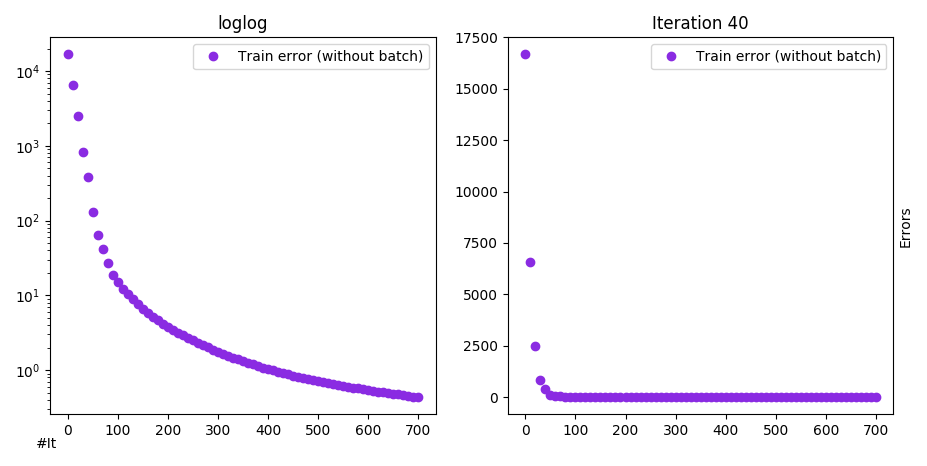
\includegraphics[scale=0.45]{Cost_Evolution_:_loglog_and_lin.png}
	\end{figure}
\end{frame}

\begin{frame}{Graph architecture}
	Graph with \red 6 hidden layers \bk with \red 80 hidden nodes \bk in each. Adam optimizer (better and the most used in literature) and \navy Lasso \bk cost function.\\
	
	TensorFlow graph that can be visualized with Tensorboard :
	
	\begin{multicols}{2}	
		\noindent		
		\begin{figure}[H]
		\centering
		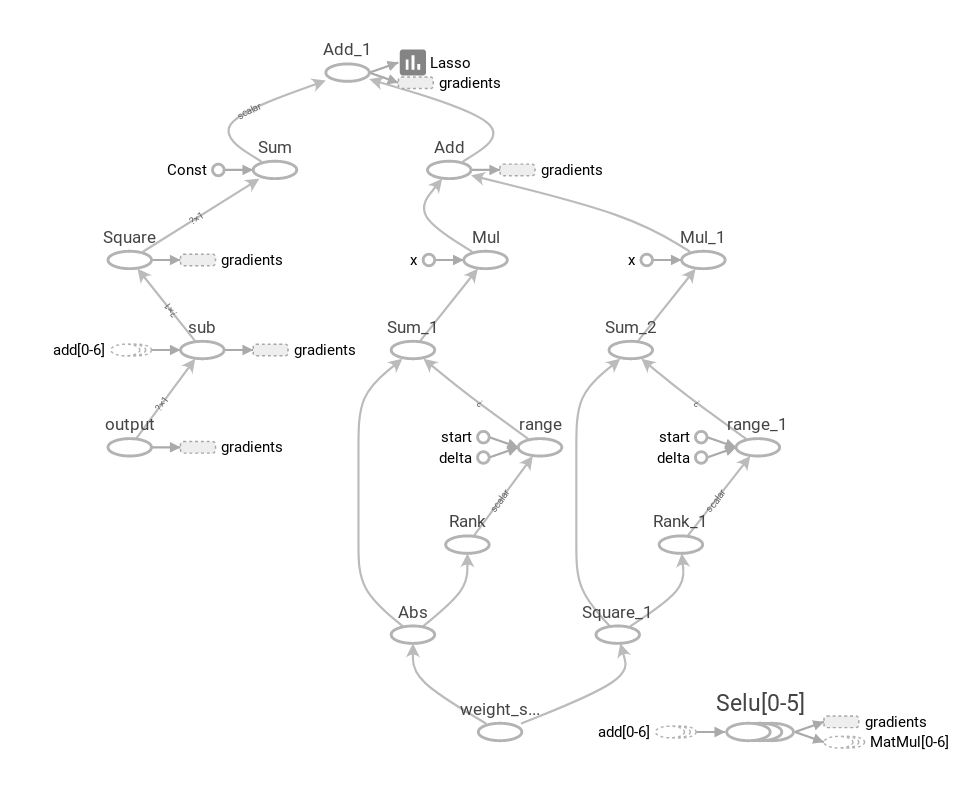
\includegraphics[scale=0.2]{Graphs.png}
		\end{figure}
	
	\columnbreak
		\centering
		\vspace{1cm}
		\begin{itemize}
			\sarrow \footnotesize Lasso = $\norm{ y_{\text{tr}} - y_{\text{pred}}}^2_{L_2} + \lambda \norm{w}_{L_1}$		 \\[1.5cm]
		
			\sarrow Activation function : selu
			\begin{figure}[H]
			\centering
			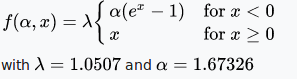
\includegraphics[scale=0.3]{SELU.png}
			\caption{From Wikipedia}
			\end{figure}
		
		\end{itemize}
	\end{multicols}
\end{frame}

\begin{frame}{Brute Force on VBE 1D I}
	New initial velocity field (first we deal with the \color{orange} orange \bk one) : 
	\begin{figure}[H]
	\centering
	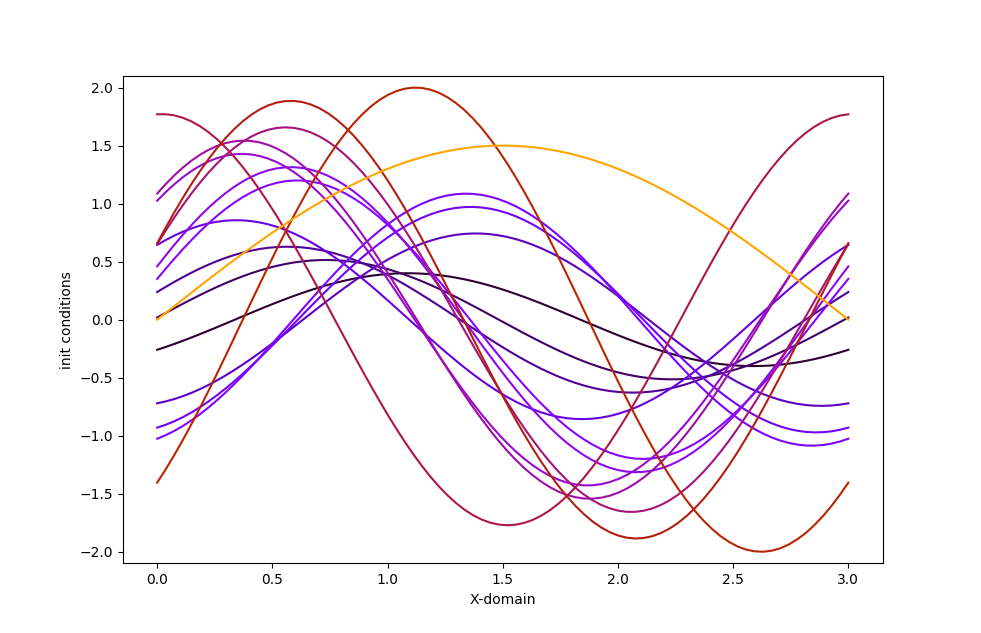
\includegraphics[scale=0.4]{Initialisation_cases_Andu1.png}
	\end{figure}
\end{frame}

\begin{frame}{Brute Force on VBE 1D I}
	\begin{figure}[H]
	\centering
	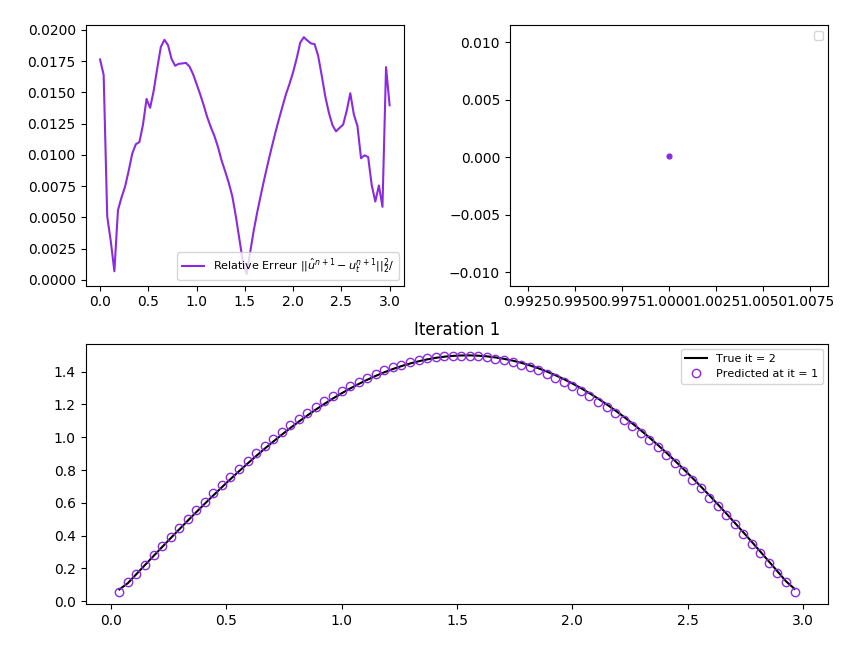
\includegraphics[scale=0.4]{Pres_First_Iteration_1.png}
	\end{figure} 
\end{frame}

\begin{frame}{Brute Force on VBE 1D I}
	\begin{figure}[H]
	\centering
	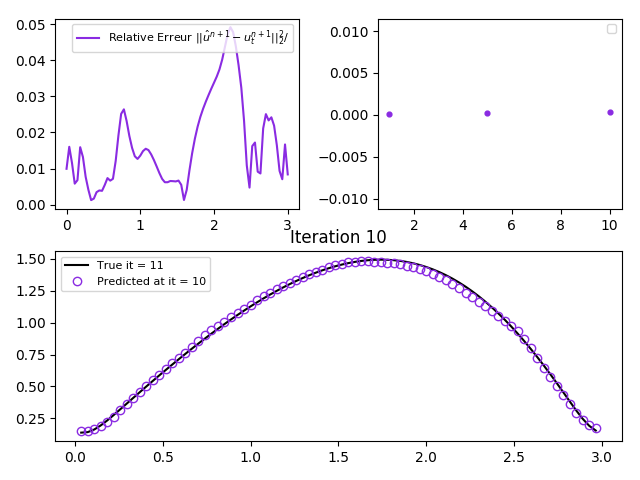
\includegraphics[scale=0.5]{Pres_Tenth_Iteration_1.png}
	\end{figure} 
\end{frame}

\begin{frame}{Brute Force on VBE 1D I}
	\begin{figure}[H]
	\centering
	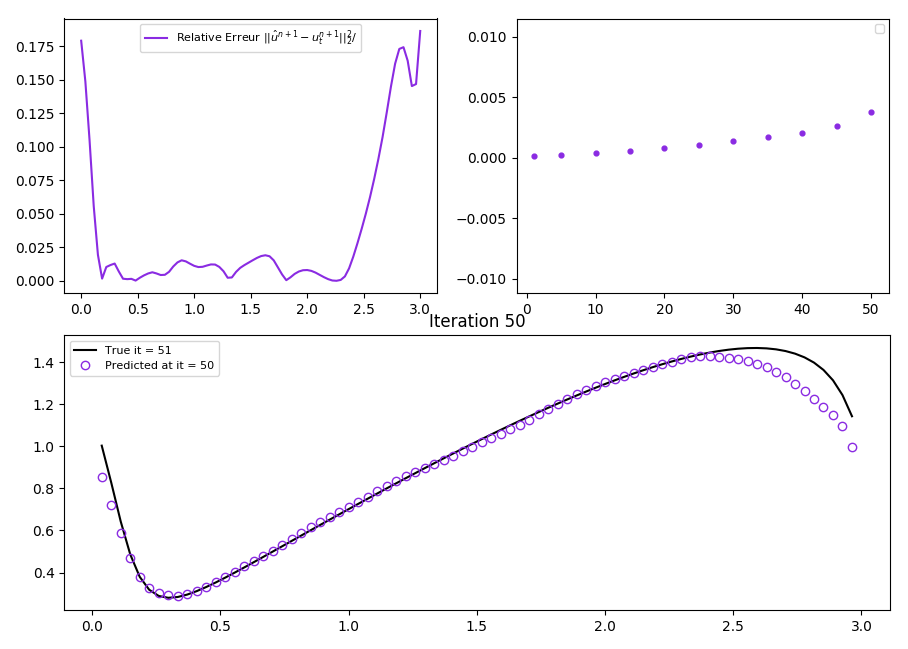
\includegraphics[scale=0.35]{Pres_50th_Iteration_1.png}
	\end{figure} 
\end{frame}

\begin{frame}{Brute Force on VBE 1D I}
	\begin{figure}[H]
	\centering
	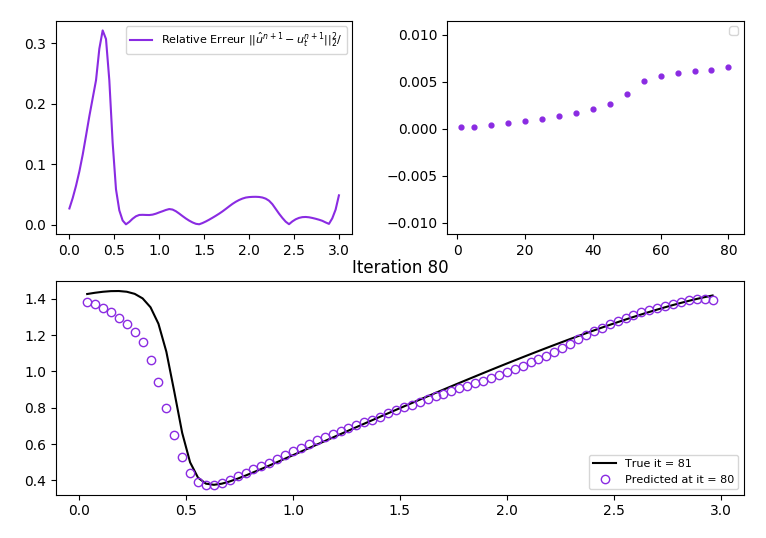
\includegraphics[scale=0.42]{Pres_Last_Iteration_1.png}
	\end{figure} 
\end{frame}

\begin{frame}{Brute Force on VBE 1D II}
	New initial velocity field (we deal now with the \color{cyan} cyan \bk one) : 
\vspace{-0.3cm}	
	\begin{figure}[H]
	\centering
	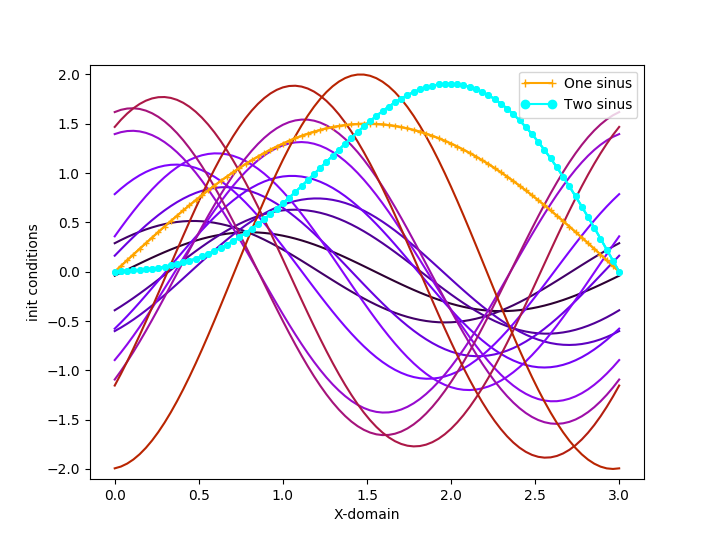
\includegraphics[scale=0.5]{Initialisation_cases_Last.png}
	\end{figure}
\end{frame}

\begin{frame}{Brute Force on VBE 1D II}
	\begin{figure}[H]
	\centering
	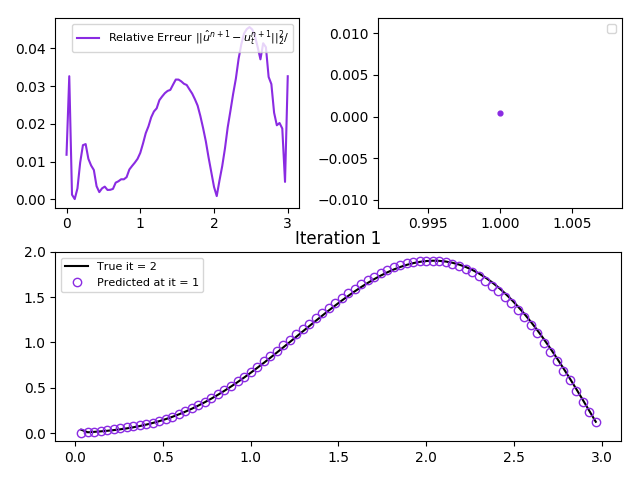
\includegraphics[scale=0.5]{Pres_First_Iteration_2.png}
	\end{figure} 
\end{frame}

\begin{frame}{Brute Force on VBE 1D II}
	\begin{figure}[H]
	\centering
	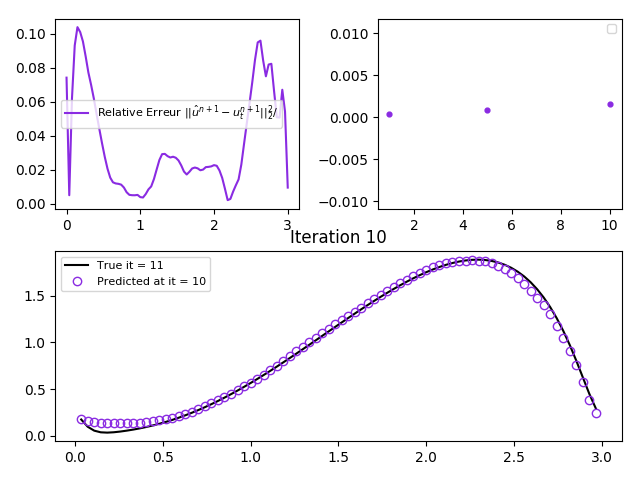
\includegraphics[scale=0.5]{Pres_Tenth_Iteration_2.png}
	\end{figure} 
\end{frame}

\begin{frame}{Brute Force on VBE 1D II}
	\begin{figure}[H]
	\centering
	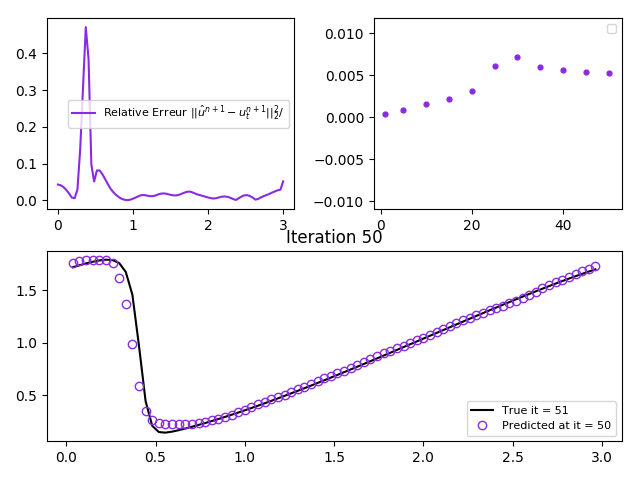
\includegraphics[scale=0.5]{Pres_50th_Iteration_2.png}
	\end{figure} 
\end{frame}

\begin{frame}{Brute Force on VBE 1D II}
	\begin{figure}[H]
	\centering
	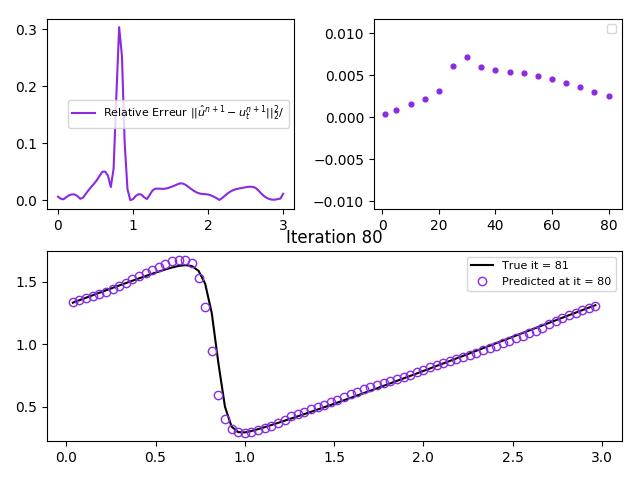
\includegraphics[scale=0.5]{Pres_Last_Iteration_2.png}
	\end{figure} 
\end{frame}

\begin{frame}{Conclusion on Brute Force}
VBE is not the simpliest equation to solve since sharp chocs
	\begin{block}{Still can be improved}
		\begin{itemize}
			\item[$\bullet$] Good approximations but can be better
			\item[$\bullet$] Accumulative errors phenomena that impose to differ local error (on the on going iteration) and global errors (accumulated through time iterations)
			\item[$\bullet$] Genetic Algorithm can be used to get the best architecture but the possible features are infinite \\[0.5cm]
		\end{itemize}
	\end{block}

	\begin{exampleblock}{Solution : Learn !}
	The solution is to use Reinforcement learning to learn the physics
	\begin{itemize}
		\item[\checkmark] Auto ajust weights given an environment 
		\item[\checkmark] Ensure to respect conservation physics law
		\item[\checkmark] Auto adjust global and local error
	\end{itemize}
	\end{exampleblock}
\end{frame}

\begin{frame}{OnGoing Deep ReiL Framework}
	
	\begin{itemize}
		\item[$\bullet$] Deep Reinforcement Learning (DQL) code in ealy stage of test.
		\item[$\bullet$] A strategy has been established and wait to be tested
		
		\item[$\bullet$] More soon .. ;)
		
	\end{itemize}

\end{frame}
\begin{frame}
\begin{center}
	\color{FireBrick} \textbf{\textit{\Large{Thank you for your attention}}} \bk
\end{center}
\end{frame}

\begin{frame}
\bibliographystyle{apalike}
\bibliography{bibliotheque}
\end{frame}

\end{document}